\begin{flushleft}

\begin{figure}[h!]
	\centering
	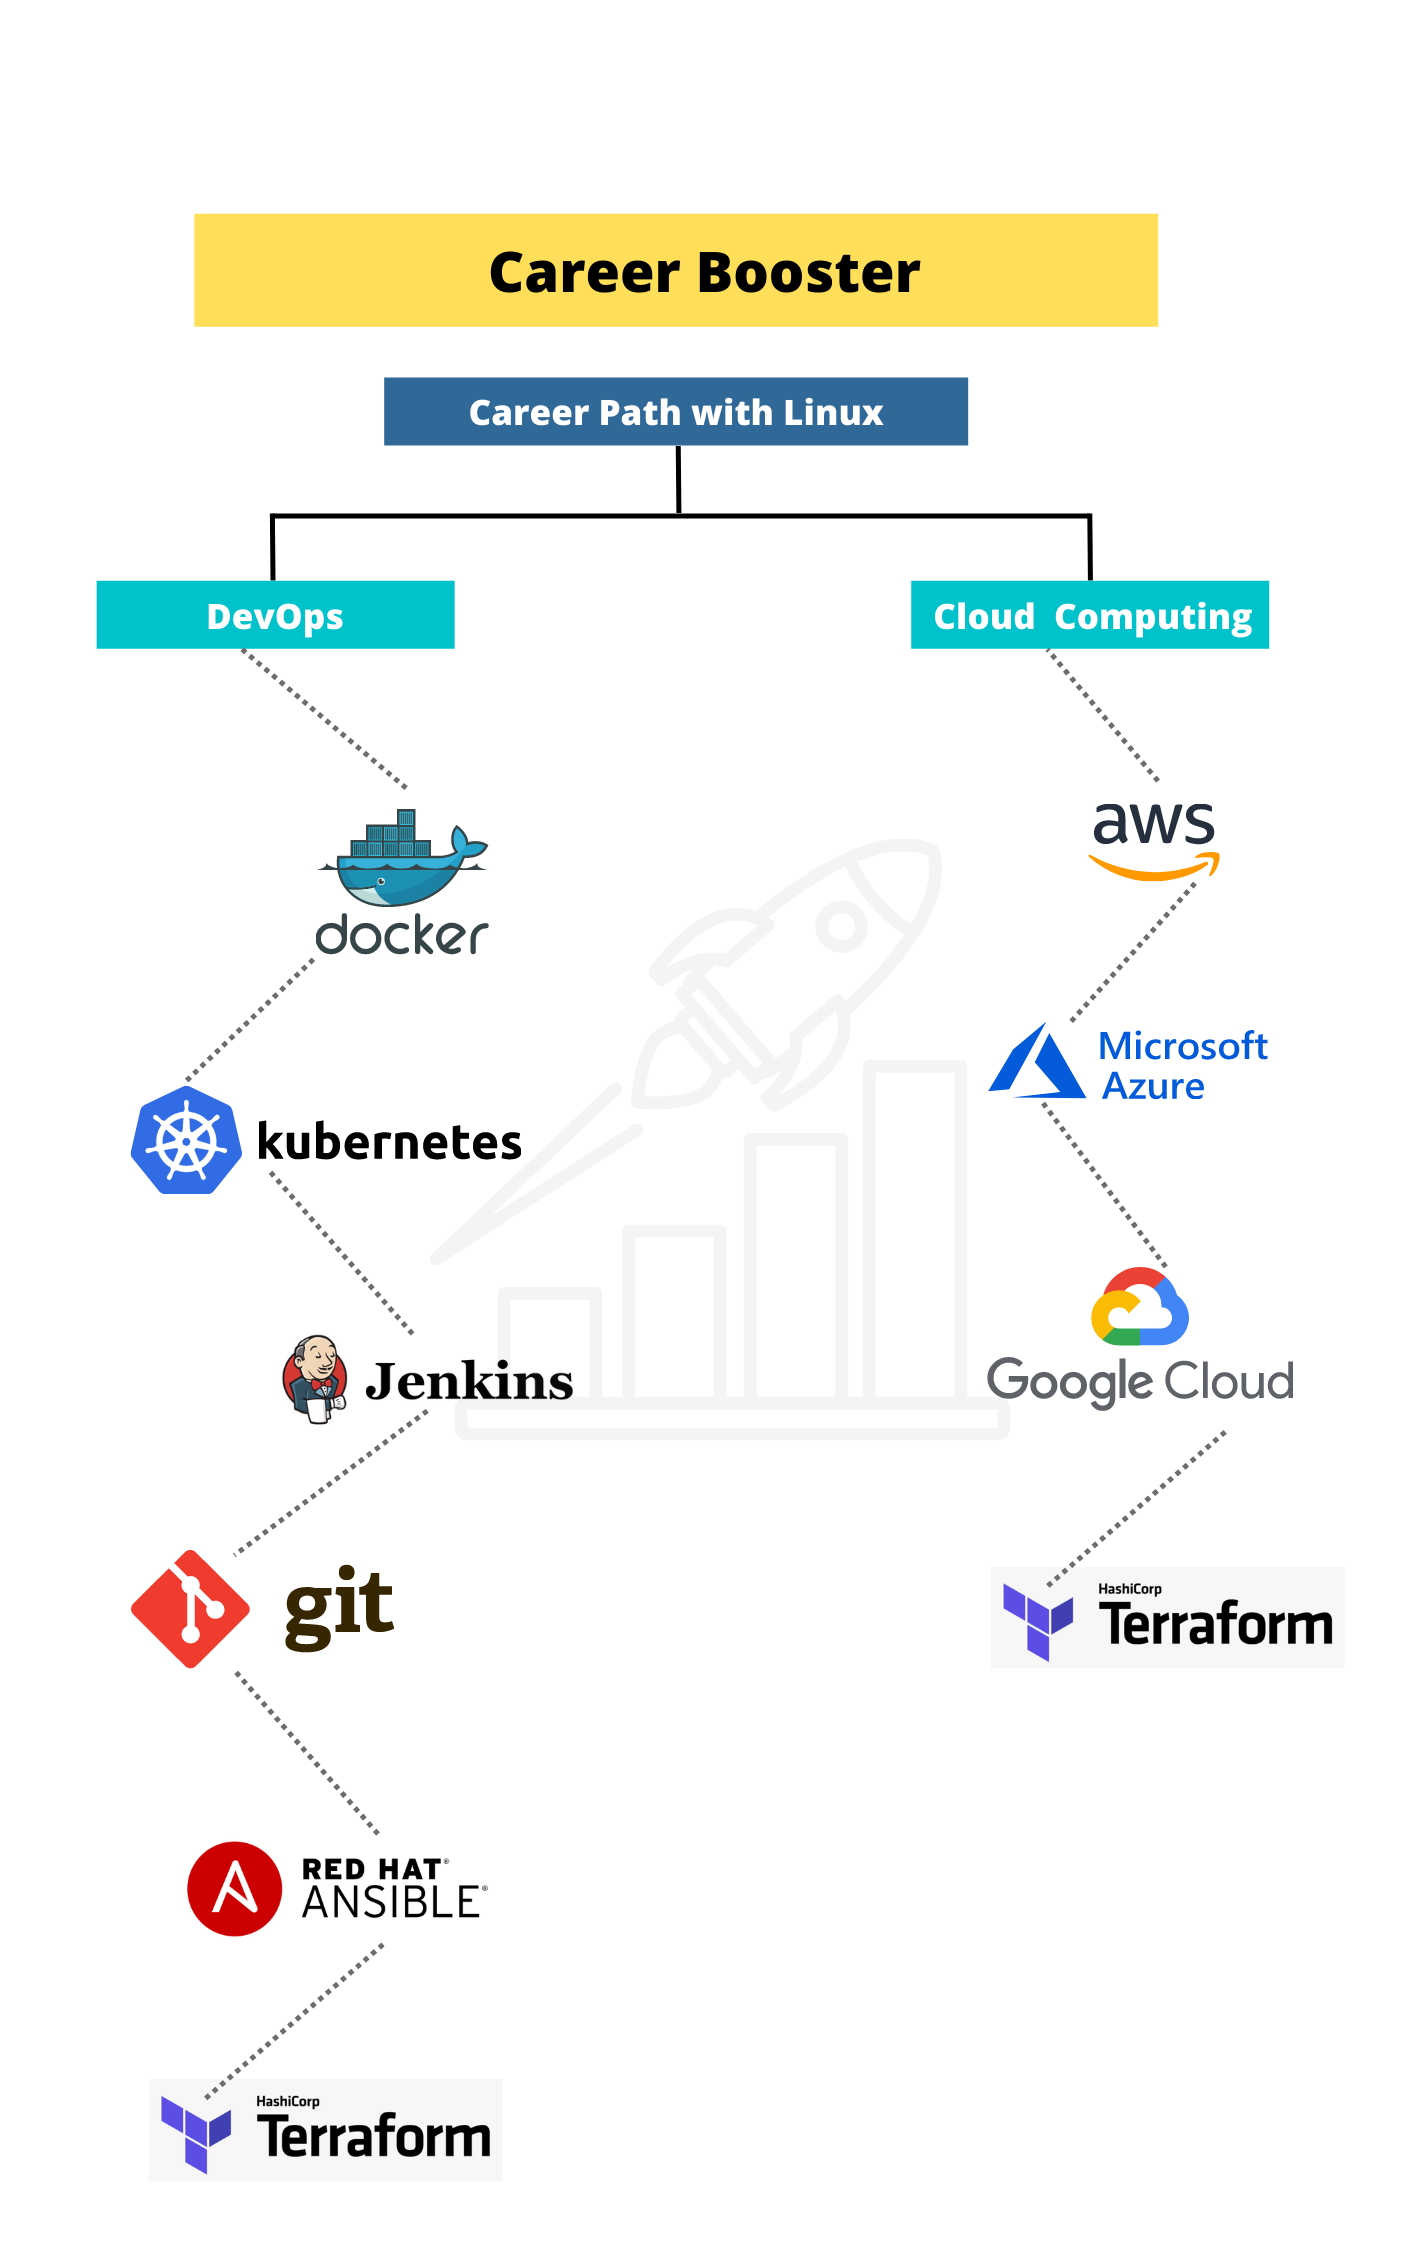
\includegraphics[scale=.35]{content/chapter1/images/career.png}
\end{figure}

\newpage
\paragraph{Linux Job Titles}
\bigskip
\bigskip
When you're looking for Linux jobs you can earn different job titles. Here are a few to watch out for:
\begin{itemize}
	\item Linux Administrator
	\item Linux System Administrator
	\item Linux System Engineer
	\item Linux Engineer
	\item Operations Engineer
	\item SRE (Site Reliability Engineer)
	\item DevOps Engineer
	\item Platform Engineer
	\item Sysadmin
	\item Release Engineer
	\item Build Engineer
	\item Security Administrator
\end{itemize}

There will be even more variations to the job titles when you add prefixes such as "Junior", "Senior" or "Associate" to the mix.

\end{flushleft}


\newpage
